\section{Design}
This section covers design considerations to inform subsequent development.
System specifications will be defined, and hardware purchasing will be informed.
The requirements of development will then be outlined before development commences. 

\subsection{Specification}
\label{sec:spec}
To inform design decisions, a specification of requirements will need to be 
defined, which themselves are informed by the aims in \cref{sec:aim} 
and research in \cref{sec:litrev}. This specification will cover a limited 
scope of the defined fundamentals and a selection of improvements and production,  
thereby limiting the reach of the project to ensure it remains feasible. 
This may be revisited if development is ahead of schedule. 

\subsubsection{Reporting}
The product will require a \gls{lora} radio modem and \acrshort{gps} receiver in order 
to obtain and transmit location. 

\paragraph{Timing}
\label{sec:timing}
A minimum transmission period of \qty{30}{\s} will be defined, however this 
likely can be greatly improved upon. Any gaps in live location should not be any greater 
than \qty{300}{\second}. 

\paragraph{Distance}
The tracker should be suited for, at worst case, a dense urban environment, 
and sufficiently capable to report information up to at least \qty{300}{\m},
given the roaming range of a cat\footnote{
    \Cref{sec:roam}.
} and the quoted values by competitors products\footnote{
    \Cref{sec:litsim}.
}.

\subsubsection{Portability}
With the primary target being cats, the product cannot be a significant burden to wear.
Portability in this case means four things:  
\begin{enumerate}
    \item Small form-factor.
    \item Lightweight.
    \item Battery powered.
    \item Attachable.
\end{enumerate}

\paragraph{Small form-factor}
The product needs to be small enough to fit on a cat. Given the likelihood for 
an outdoor cat to be squeezing through tight spaces, the product needs to be small 
enough to not get caught and become a restriction. 

The smallest form-factor will be aimed for, and designed in such a way 
that it can integrate in a seamless fashion with the cat's wearable 

As reasonable figure to start with would be dimensions of 
\qtyproduct{50 x 70 x 10}{\mm}.

\paragraph{Lightweight}
There is no clear answer for what an appropriate weight for the product 
would be given great range in the weight of a cat. The range easily covers
\qty{3}{\kg} to \qty{6}{\kg} for healthy pet cats \cite{kienzle:pilot}.

The answer to how much weight a cat can carry for long periods is even 
less clear. Anecdotal evidence suggests a value of around 10\%
is easily manageable. With that in mind, an aim for 
half that at, 5\% of the minimum likely weight (\qty{3}{\kg})
is a reasonable value, such that the weight is appropriate for any cat.
This puts the desired weight for the tracker at $\leq \qty{150}{\g}$, 
subject to testing to validate.

\paragraph{Battery powered}
\label{sec:specsbatt}
The key factor of portability is that the product can operate 
without a direct connection to an outlet for power. 
This means that the product requires some form of portable power.

With convenience, environmental, and energy-density (and thereby weight) considerations in mind \cite{blomgren:lithium},
the most appropriate type of battery will be rechargeable lithium-ion. This may raise some safety concerns 
due to the high likelihood of flammability of rechargeable battery cells \cite{chen:flammable}.

The most pertinent question is how long should such a battery allow the tracker to operate.
An outdoor domestic cat spends an average of \qty{8.4}{\hour} outdoors \cite{Bischof2022},
this puts a minimum value of \qty{9}{\hour} of supply necessary. 

\paragraph{Attachable}
Some method to attach the product to a cat needs to be devised. 
If it is small enough, this may be on a collar. Alternatively, 
attached to a vest may also work. This is very dependent on the 
dimensions the product takes in the end. 
Furthermore, if the product takes a prominent, protruding shape,
it needs to detach easily so as not to be a restriction for the animal.

The primary focus will be on ensuring it cannot be caught in anything to
begin with, as the tracker coming loose defeats its purpose.


\subsubsection{Suitability}
This product is designed for use by the average pet owner. Therefore, no 
specialised knowledge on how to operate any equipment can be expected. 
Furthermore, the system should be installable and maintainable using 
skills and hardware the average household can be expected to own, with some 
allowances for a small amount of DIY work. 

\paragraph{Installable}
If any hardware requires installation, it must be in as simple a manner as 
possible, with only basic (manual) tools. The expectation will be that installation
should be, at most, as difficult as a simple piece of furniture
 from a DIY store. 

\paragraph{Compliance}
Compliance for consumer products needs to be met. If certification
is not explicitly sought (for example, in the case third-party verification 
is required), the product must still meet the standards outlined such 
that it can be certified when necessary.

As a product developed in the UK, UKCA guidelines will be used. 


\subsubsection{Reliability}
The reliability of the tracker will be a matter of concern, 
as it would be especially inappropriate for it to fail in its reporting 
midway. 
\paragraph{Stable}
Part of the product relies on correct handling and processing of 
information over code. When interpreting data sets, poorly formatted 
data has the tendency to cause crashes in unsafe code. 
The code will need to be built to safely handle errors, both in the 
above-mentioned case and in any other potential points of 
software failure. 

When an error occurs, it will need to report the error and then 
continue execution with minimal downtime. Where the fault is fatal for whatever reason, 
sufficient diagnostic information is required so that fault-finding 
can be facilitated. 

\paragraph{Fault resistant}
In continuation with safely handling software errors, the 
hardware will also need to be fault-tolerant. This 
inclusively includes problems 
that may occur due to inclement weather or impacts.

\paragraph{Repairable}
Where such a hardware fault occurs that the product is no longer 
functional, repairs are to be facilitated in reasonably easy manner. 
The user should have the facilities to perform simple repairs, like 
changing an ageing battery. 
More complex repairs that require tools or specific knowledge
will be carried out by a trained individual, and therefore out of 
scope. However, a user with sufficient knowledge should not 
be hindered from performing repairs themselves if they are able. 

\paragraph{Safety}
This product introduces flammable electronics to wet environments, 
and therefore must be designed such that delicate parts are protected 
from the elements and, should such exposure occur, not be an 
inherent fire or electrocution risk.

\paragraph{Deduplication}\label{sec:dedupe}
Given that all transmissions will be operating on the same frequency, 
data from different trackers will be received by any given antenna, 
of which, the unsuitable data will need to be filtered out.  
This also brings up the question of security and `listening in' on 
another's pet. 

\subsection{System overview}
The system can be broken down into two independent parts - the `transmitter' (attached to the cat)
and `receiver' (stationary at the owner's home). Each subsystem has an independent process of operation.
The minimum requirements are subsequently outlined in \cref{fig:system overview flowchart}.

\begin{figure}[H]
    \centering
    \begin{subfigure}{.4\textwidth}
        \centering
        \begin{tikzpicture}
            \node (start) [startstop] {Start};
            \node (timer) [process, below of=start, yshift=-0.6cm] {Start timer};
            \node (loc) [process, below of=timer, yshift=-0.6cm] {Get location};
            \node (elapse) [process, below of=loc, yshift=-0.6cm] {30s elapsed};
            \node (emit) [io, below of=elapse, yshift=-0.6cm] {Emit location};

            \draw [arrow] (start) -- (timer);
            \draw [arrow] (timer) -- (loc);
            \draw [arrow] (loc) -- (elapse);
            \draw [arrow] (elapse) -- (emit);
            \draw [arrow] (emit) -- ++(2.5,0) |- (loc);
        \end{tikzpicture}
        \caption{Transmitter}
    \end{subfigure}\quad
    \begin{subfigure}{.4\textwidth}
        \centering
        \begin{tikzpicture}
            \node (start) [startstop] {Start};
            \node (inp) [io, below of=start, yshift=-0.6cm] {Await location};
            \node (store) [process, below of=inp, yshift=-0.6cm] {Store location};

            \draw [arrow] (start) -- (inp);
            \draw [arrow] (inp) -- (store);
            \draw [arrow] (store) -- ++(2.5,0) |- (inp);
        \end{tikzpicture}
        \caption{Receiver}
    \end{subfigure}    
    \caption{System overview flowchart}
    \label{fig:system overview flowchart}
\end{figure}

\subsection{Hardware}

Given the specification list, some hardware requirements can be defined to inform purchasing decisions.
The transmitter needs to be portable, therefore each component is size, weight, and power limited. The receiver,
on the other hand, is designed to be stationary and has no technical size or power limitations. However, 
it has to be sized within reason for a product designed for home use.

The following component list will help inform what specific components are required, which has been 
drawn into a hardware block diagram in \cref{fig:hardwareblockdiag} to aid visualisation. 
\begin{itemize}
    \item Transmitter
          \begin{itemize}
              \item \acrshort{gps} module for location.
              \item \gls{lora} module for transmission.
              \item Small form-factor antenna to aid transmission.
              \item Microcontroller for general computation.
              \item Battery as a remote power source.
          \end{itemize}
    \item Receiver
          \begin{itemize}
              \item \gls{lora} module for transmission.
              \item Microcontroller or \acrshort{sbc} for computation.
          \end{itemize}
\end{itemize}

% \begin{figure}[htbp]
%     \centering
%     \begin{subfigure}[b]{0.475\textwidth}
%         \centering
%         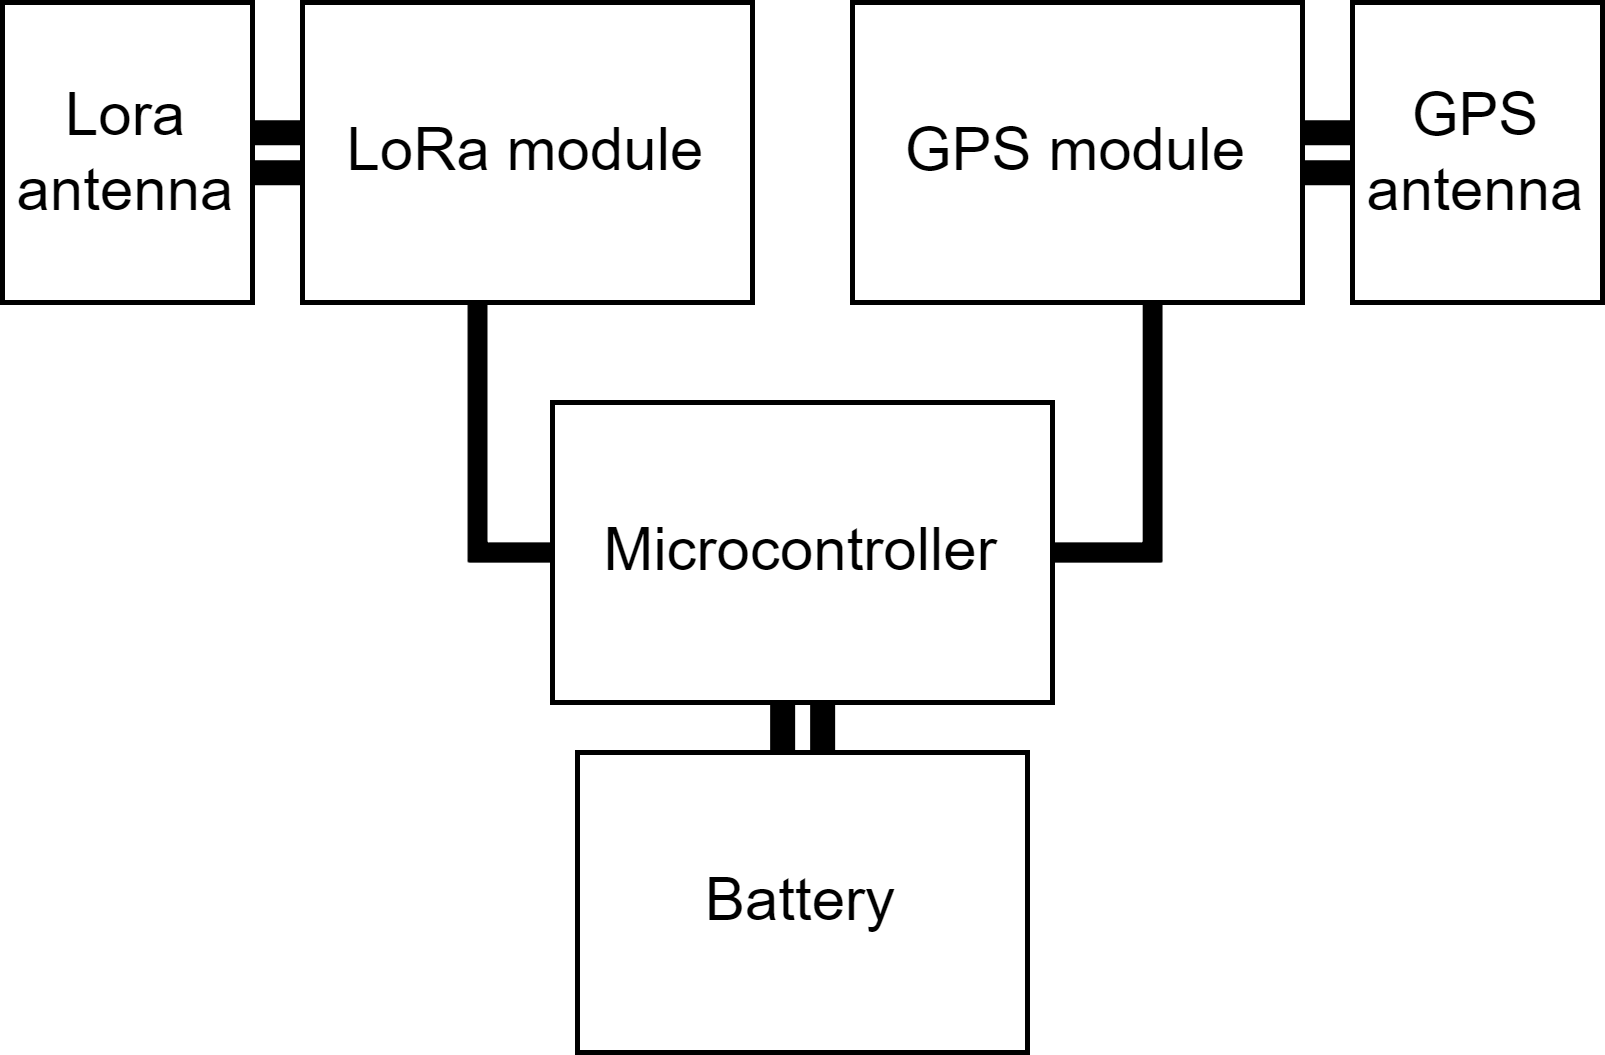
\includegraphics[height=5cm, keepaspectratio]{../figures/mcblock.png}
%         \caption{Transmitter}
%     \end{subfigure}
%     \hfill
%     \begin{subfigure}[b]{0.475\textwidth}
%         \centering
%         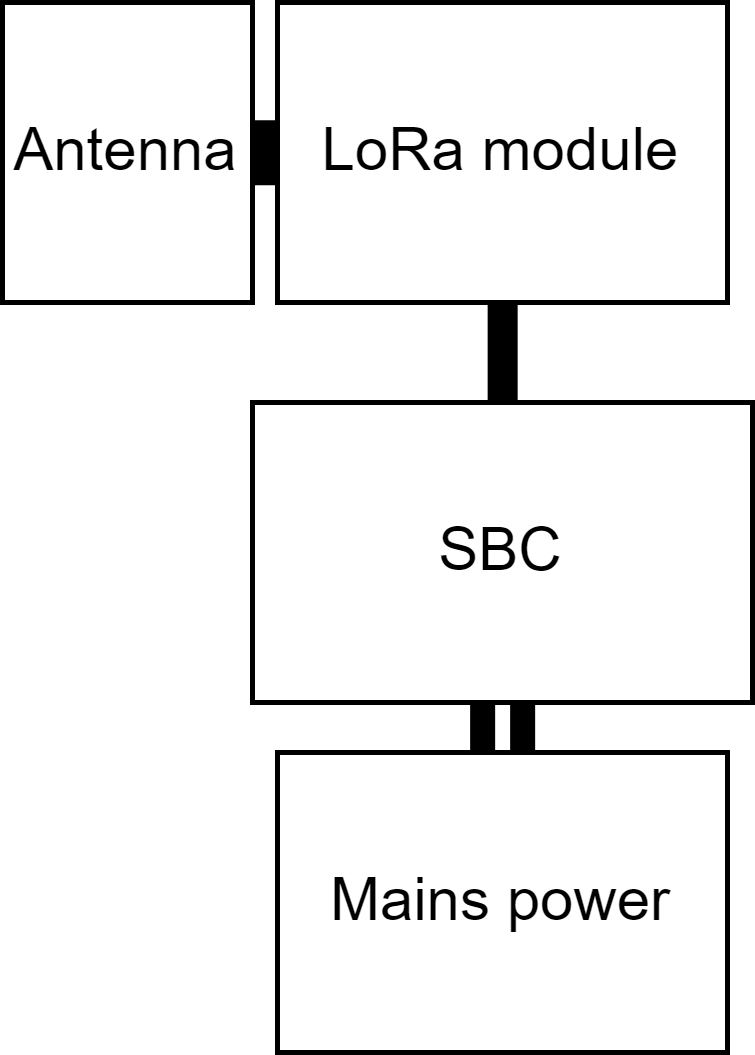
\includegraphics[height=5cm, keepaspectratio]{../figures/sbcblock.png}
%         % \includesvg[inkscapelatex=false,width=\textwidth]{../figures/sbcblock.svg}
%         \caption{Receiver}
%     \end{subfigure}
%     \caption{Hardware block diagram}
%     \label{fig:hardwareblockdiag}
% \end{figure}

\begin{figure}[H]
    \centering
    \begin{subfigure}[b]{0.625\textwidth}
        \centering
        
        \begin{tikzpicture}        
            \node (mc) [rec] {Microcontroller};
            \node (lora) [rec, above of=mc, yshift=0.6cm, xshift=-1.25cm] {LoRa\\module};
            \node (loraant) [rec, left of=lora, xshift=-1.5cm] {LoRa\\antenna};            
            \node (gps) [rec, above of=mc, yshift=0.6cm, xshift=1.25cm] {GPS\\module};
            \node (gpsant) [rec, right of=gps, xshift=1.5cm] {GPS\\antenna};
            \node (batt) [rec, below of=mc, yshift=-0.6cm] {Battery};

            \draw [bar] (mc) -- (lora);
            \draw [bar] (lora) -- (loraant);
            \draw [bar] (mc) -- (gps);
            \draw [bar] (gps) -- (gpsant);
            \draw [bar] (batt) -- (mc);
        \end{tikzpicture}

        \caption{Transmitter}
    \end{subfigure}
    \hfill
    \begin{subfigure}[b]{0.325\textwidth}
        \centering
        \begin{tikzpicture}        
            \node (sbc) [rec] {SBC};
            \node (lora) [rec, above of=sbc, yshift=0.6cm] {LoRa\\module};
            \node (loraant) [rec, left of=lora, xshift=-1.5cm] {LoRa\\antenna};   
            \node (pwr) [rec, below of=sbc, yshift=-0.6cm] {Mains\\power};

            \draw [bar] (sbc) -- (lora);
            \draw [bar] (lora) -- (loraant);
            \draw [bar] (pwr) -- (sbc);
        \end{tikzpicture}      

        \caption{Receiver}
    \end{subfigure}
    \caption{Hardware block diagram}
    \label{fig:hardwareblockdiag}
\end{figure}

There are many possible configurations to produce the sets of hardware required 
from parts available across different vendors. With this in mind, solutions that 
incorporate built-in features will be prioritised.

\subsubsection{SBC choices}
Some decisions were made to narrow down the diverse range of options, given hardware 
availability and technological experience. Regarding the transmitter controller;
while this may be as simple as a microcontroller, with extensibility and future-proofing 
in mind\footnote{
    For example, serving a user-interface, storing data in a database etc.
}, an \acrshort{sbc} will be the product of focus. Given hardware shortages,
should there be none available, this may be revisited. 
There are a number of \acrshort{sbc} offerings available, some of which are listed 
with a discussion in \cref{table:sbc}.

{\small
\begin{xltabular}{\linewidth}{|Z|Z|Z|Z|}
    \hline
    \rowcolor{tableh2}
    Board & Description & Benefits & Drawbacks \\
    \hline
    Raspberry Pi        & A series of general purpose \acrshortpl{sbc} using Broadcom BCM series \acrshortpl{soc}. 
        & \textbullet Inexpensive \newline \textbullet \acrshort{gpio} \newline \textbullet Pi 3 available
        & \\
    \hline
    NVIDIA Jetson Nano  & AI and neural network development focused, built around the ARM Cortex-A57 and NVIDIA Maxwell.                                       
        & \textbullet Powerful \newline \textbullet \acrshort{gpio}
        & \textbullet Expensive \newline \textbullet More powerful than necessary \newline \textbullet Availability \\ 
    \hline
    Beaglebone Black    & Pi equivalent, using an ARM Cortex-A8.                              
        & \textbullet Inexpensive \newline \textbullet \acrshort{gpio}
        & \textbullet Availability \\
    \hline
    Dell Wyse           & Thin client server/PC.
        & \textbullet Familiar interface for an end user \newline \textbullet Easier \acrshort{gui} programming  
        & \textbullet No \acrshort{gpio} \newline \textbullet Very expensive \\
    \hline
    \caption{\Acrshort{sbc} considerations}\label{table:sbc}
\end{xltabular}
}

With all things considered, the Raspberry Pi is the most obvious choice simply
from the standpoint that a Pi 3 is currently available for use. 
Given the current climate, it is virtually impossible to order computing hardware in this category. Even the Pi Compute
Modules, small form-factor Pi boards with no peripherals or breakouts, are often out of stock. This is despite the fact that 
these boards are unable to function `out of the box'. 

\subsubsection{Microcontroller choices}
The transmitter does not need to perform anything greater than obtaining \acrshort{gps} coordinates 
and transmitting them by \gls{lora} radio. For this reason, a microcontroller is well suited. 
There is an even greater selection available than with the \acrshort{sbc} choices. Therefore, 
as before, the options will be shortlisted and considered in \cref{table:mc}.
\clearpage

{\small
\begin{xltabular}{\linewidth}{|Z|Z|Z|Z|}
    \hline
    \rowcolor{tableh2}
    Board & Description & Benefits & Drawbacks \\
    \hline
    Arduino Uno & One of the most popular microcontrollers available, with an ATmega328P at its core. 
        & \textbullet Widely available \newline \textbullet Large peripheral and software support 
        & \textbullet Large \\
    \hline
    Challenger RP2040 LoRa & Embedded computer with integrated LoRa modem using the RP2040, a dual ARM Cortex-M0+ microcontroller. 
        & \textbullet Integrated \gls{lora} modem 
        & \\
    \hline
    Feather RP2040 & RP2040 board produced by Adafruit in the feather form-factor.
        & \textbullet Feather form-factor \newline \textbullet USB-C
        & \\
    \hline
    Wio-E5 mini & Compact LoRa dev board produced by Seeed Studio using an STM32WLE5JC, a bundled ARM Cortex-M4 microcontroller and SX126X \gls{lora} radio modem.
        & \textbullet Integrated microcontroller and \gls{lora} modem \newline \textbullet USB-C
        & \textbullet Availability \newline \textbullet Involved programming requirements\\
    \hline
    Feather 32u4 with LoRa & Feather form-factor board with LoRa produced by Adafruit, sporting an ATmega32u4.
        & \textbullet Integrated \gls{lora} modem \newline \textbullet Prior experience \newline \textbullet Feather form-factor
        & \textbullet Availability \\
    \hline
    \caption{Microcontroller considerations}\label{table:mc}
\end{xltabular}
}

The board of choice here would be the Feather RP2040. While integrated \gls{lora} 
is certainly beneficial, having the flexibility to customise it during development 
may prove more helpful\footnote{
    The RFM95W \gls{lora} chipset uses \acrshort{spi} and has, in previous experience,
caused difficulties with hardware on the same bus. In case it is necessary, an alternative set
of hardware using the \acrshort{i2c} bus will be produced.
}. Furthermore, this board shares the advantage of other Feather 
boards in that they are stackable, meaning Adafruit's large range of peripherals 
(including \gls{lora} Featherwings and \acrshort{gps} Featherwings) are available to use. 

Purchasing two such \gls{lora} Featherwings for use in the transmitter and receiver 
ensures they are able to communicate with each other without issue. Given the selected 
form-factor and subsequent ease of use, it follows that the \acrshort{gps} module will be 
from Adafruit's Featherwing line. 

\subsection{Purchasing}

Some antenna options will be included as the best approach 
for this has not yet been determined. Ceramic antennae have the smallest form-factor,
however they may prove difficult to mount due to small contact points compared to more traditional 
wire antennae. The receiver will also require a large gain antenna to pick up weak transmissions.

A preliminary hardware set was produced\footnote{
    \Cref{table:prelimhardwarelist}.
}. This list consists 
of two sets of hardware for the transmitter, hardware required regardless of set, and some antenna 
options. 

The radios selected use the same model modem, the RFM95W \cite{hoperf:rfm95w}, 
ensuring the modules are capable of communicating (i.e. are operating within the 
same wavelength range).

\paragraph{Order review}
The list had to be adjusted to primarily target hardware from approved vendors\footnote{
    \Cref{table:updatedhardwarelist}.
}. 
With the vendor adjustment made, some of the initial hardware had to be substituted for 
more expensive alternatives. This made board options simpler by limited the feasible solution
to a Feather M0 with bundled \gls{lora} modem. Additional accessories were included, along with 
an extensive set of antenna and battery options to choose from. 

This list was further adjusted to omit spare hardware that is available to use (for example, 
headers, connectors, etc.). Furthermore, battery purchasing will be put on hold until 
the required capacity can be determined. Finally, the \gls{lora} module for the Pi was 
changed to a \acrshort{hat}. This uses the same radio hardware, but has the additional benefit 
of being able to directly interface with the Pi pins. 
The list was then requested for purchasing. 


